\section{The Benchmarx Framework}
\label{sec:Benchmarx}

%\NOTE{\emph{Length:} 2 p., \emph{Responsible:} Thomas}
%
%\NOTE{Overview of the framework, provided components, approach to tool integration, synchronization dialogues, design and classification of test cases, execution of test cases.}
%\subsection{Overview}

\begin{figure}[tb!]
	\centering
	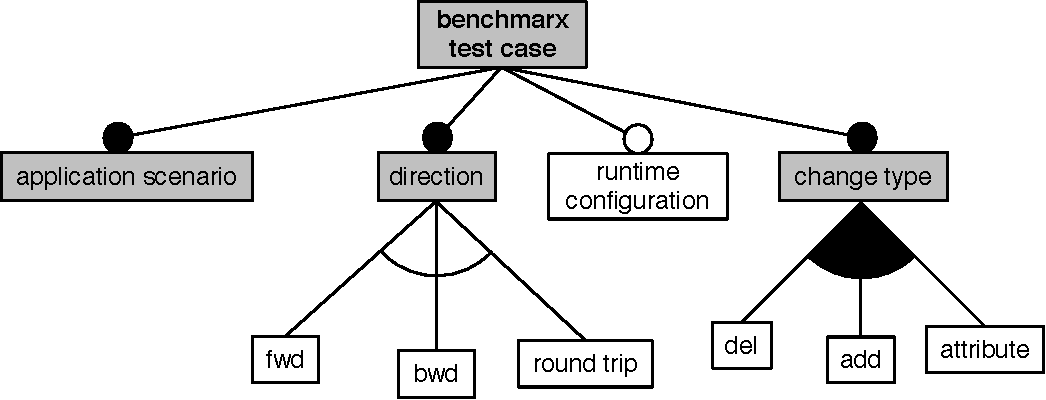
\includegraphics[width=\columnwidth]{diagrams/framework/feature-model-benchmarx-test-case}
	\caption{Variability of benchmarx test cases}
	\label{fig:featureModelBenchmarxTestCase}
\end{figure}

\begin{figure*}[tb!]
	\centering
	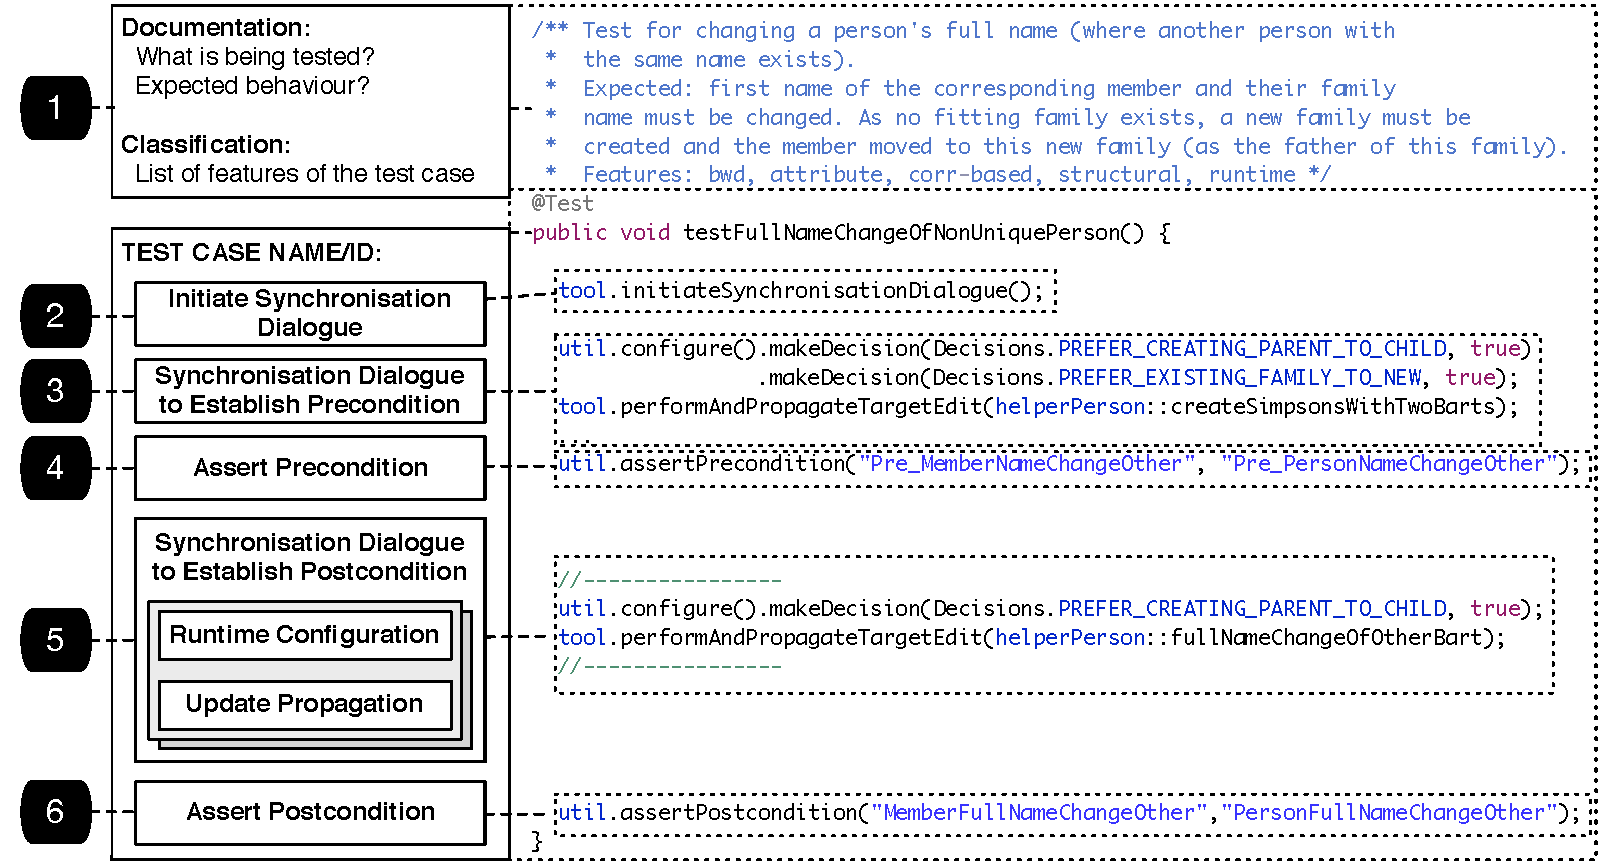
\includegraphics[width=0.75\textwidth]{diagrams/benchmarx/testCase}
	\caption{A benchmarx test case as a synchronization dialog}
	\label{fig:benchmarxTestCase}
\end{figure*}



The Benchmarx framework is a component-based framework allowing for a comparison of arbitrary bx tools. 
A major challenge that must be addressed by the framework is that different bx tools may require different input data. 
The Benchmarx framework must thus provide a unifying design space, in which different bx tool architectures can be placed, classified, and evaluated. 



While the general conceptual design of the Benchmarx framework can be transferred to any technological space, we provide a reference implementation based on Eclipse, the Eclipse Modeling Framework (EMF), JUnit as a unit testing framework, and Java.
To ensure that non-EMF and even non-JVM-based bx tools can be integrated with no restrictions on the input data of the tools, we use a string representation of produced and expected models established by convention for each benchmark example.
The current solutions to the Families-to-Persons case show that it is indeed possible to integrate diverse bx tools with reasonable effort.

\subsection{Design of a benchmarx test suite}
\label{sec:DesignOfABenchmarxTestSuite}

\begin{figure*}[tb!]
	\centering
	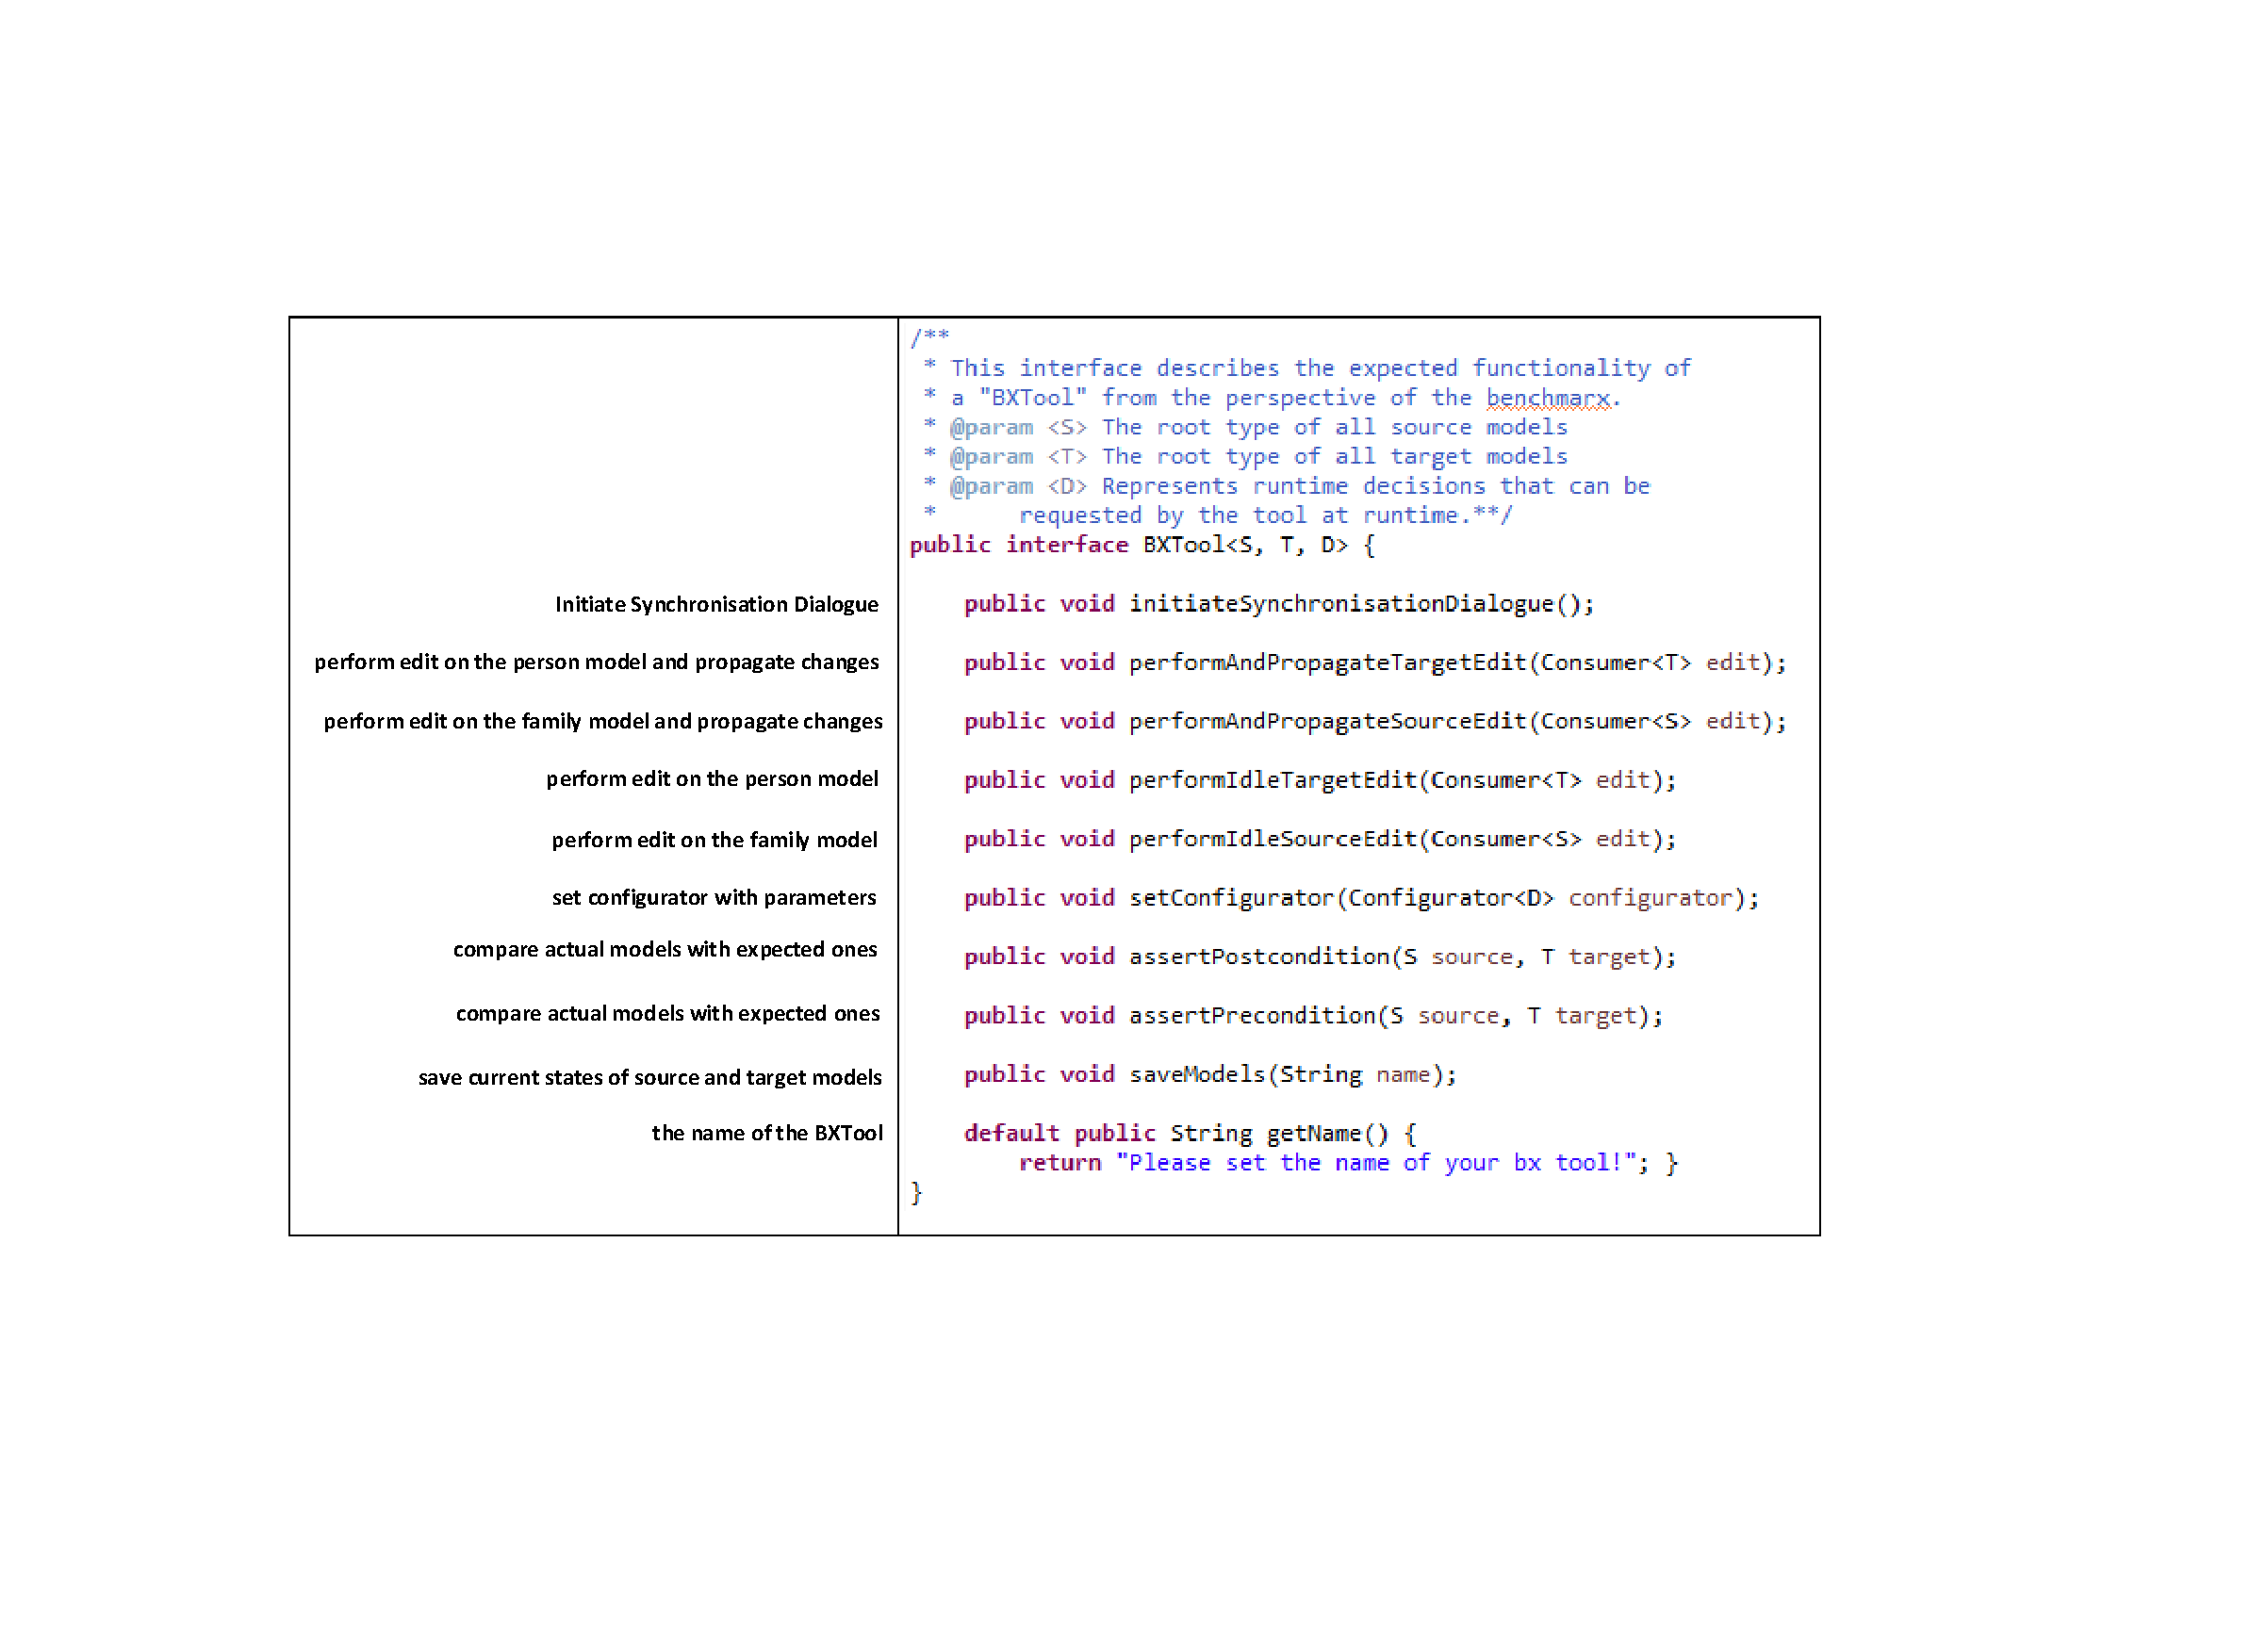
\includegraphics[width=0.75\textwidth]{diagrams/benchmarx/BXTool}
	\caption{The BXTool interface}
	\label{fig:refImplementation}
\end{figure*}

Figure \ref{fig:featureModelBenchmarxTestCase} depicts a feature model for benchmarx test cases. 
Every benchmarx test case must state the relevant application scenario (cf. Figure~\ref{fig:featureModelBxTools}), its direction to be (exclusively) \emph{fwd} (forward), \emph{bwd} (backward) or a mix of both, i.e., a \emph{round trip}, if the test case requires \emph{runtime configuration} or not, and the combination of different change types applied in the test. 
The set of possible change types can be extended in the future to accommodate more expressive frameworks. 

Benchmarx is designed as a generic framework for benchmarking bx tools; we thus strive to minimize requirements regarding the typically tool-specific representation of deltas and corrs. 
Instead of establishing some standard data structure for deltas and corrs, test cases are designed as \emph{synchronization dialogs}. 
A synchronization dialog always starts from the same agreed upon initial consistent state, and then applies a sequence of edits to the source and target models. 
Only the resulting models are directly asserted by comparing them with expected versions.
In this manner, each bx tool is free to maintain arbitrary internal state, e.g., recording deltas during edit application, or maintaining corrs in whatever format is required.

A benchmarx test case is depicted schematically to the left of Figure \ref{fig:benchmarxTestCase}, with a concrete test case for our example depicted to the right of Figure~\ref{fig:benchmarxTestCase}, following the proposed schema using JavaDoc, Java, and JUnit as implementation technologies.
Each test case contains a documentation (cf. label~1 in Figure~\ref{fig:benchmarxTestCase}) stating (i)~what is being tested, (ii)~the expected behaviour, and (iii)~a list of the concrete features of the test case taken from Figure~\ref{fig:featureModelBenchmarxTestCase} to clarify at a glance if a given bx tool can be expected to pass the test or not, i.e., if the relevant application scenario for the test case matches the addressed application scenario of the (implemented solution with the) bx tool. 

The test case itself starts by initializing the bx tool which is being tested (label~2); the agreed upon starting state is hereby established (e.g., for the Families-to-Persons benchmark this comprises a single empty family register and a corresponding single empty person register), and all necessary internal (auxiliary) tool-specific data structures can be created.

%%%%% TONY is here %%%%%>

The subsequent part of a test case (label~3) consists of a series of propagation steps, used to establish the precondition of the test. 
Although this creates a dependency on other tests (asserting exactly this precondition), it allows us to abstract from any tool-specific corr representation, as every bx tool can build up whatever internal state it requires along with the precondition. 
In this manner, the input corr is ``passed'' implicitly to the bx tool via a series of preparatory propagation steps.
Each propagation step is specified in the test case as a source or target edit (realized as a Java lambda expression), which is passed to the bx tool and is to be performed on the source or target model.
In this manner, the bx tool can record\footnote{EMF supports this via a notification framework.} whatever it wants when applying the edit to produce, e.g., a tool-specific representation of an o-delta or s-delta.

The precondition is finally asserted (label~4), representing a well-defined starting point for the test. 
If the test requires a runtime update policy (cf. section~\ref{sec:Introduction}), this is configured (label~5) just before propagating the relevant input edit.
A sequence of such (optional) configuration and edit propagation steps form the primary synchronization dialogue used to establish the postcondition (label~5).
The final part of a test case (label~6) is an assertion of the postcondition, checking if the final source and target models are as expected. 



In the concrete test case depicted to the right of Figure~\ref{fig:benchmarxTestCase}, a number of persons are created in the person register and then propagated backward to establish a consistent family register that is asserted as a precondition. 
As part of the actual test, a person named \texttt{Simpson, Bart} is now renamed in the person register; this change is propagated backward with a runtime update policy set to prefer creating parents (if possible) to creating children. 
Note that in this particular test, two persons with the name \emph{Bart Simpson} are created as part of the precondition (indicated by the target edit \texttt{createSimpsonsWithTwoBarts}). 
As a consequence, this test can only be reliably passed if corrs are exploited as explicit input (indicated by the feature \texttt{corr-based} in the classification of the test). 

The current test suite provided for the Families-to-Persons case consists of such test cases as in Figure~\ref{fig:benchmarxTestCase} separated into two broad categories: (1)~\emph{batch} test cases providing only the input model and no horizontal input (initial-batch-based), and (2)~\emph{alignment-based} test cases providing an input delta and input corr (delta-corr-based).
More tests covering the other bx application scenarios identified in Figure~\ref{fig:architectureLandscape} can be added in the future.
Each category comprises test cases for each transformation direction.\footnote{Recall from section~\ref{sec:Introduction} that the \emph{forward} direction is from the Families model to the Persons model, while \emph{backward} is from the Persons model to the Families model.}

While the batch test cases are basic tests used to check if a given source model is transformed into a new target model correctly, different input source deltas are handled by the alignment-based tests. 
In particular, renaming, deleting, and moving persons and family members are currently addressed in these test cases. 
To keep the number of test cases manageable, only the batch category contains separate test cases for each combination of configuration parameters.
In the alignment-based category, the parameters (preferences represented by the update policy) are changed dynamically during test case execution.



\subsection{Implementing a benchmark with a bx tool}



In order to use a specific bx tool with the benchmarx framework, a single interface \code{BXTool}, depicted and described in Figure~\ref{fig:refImplementation}, needs to be implemented.
For EMF-based tools, we provide an abstract class \code{BX\-Tool\-For\-EMF} that contains implementations for both \code{assert} methods and can be subclassed to simplify the integration in the benchmark.

The method \code{initiate\-Synchronisation\-Dialogue} is invoked before each test case run and is used to establish the agreed upon common starting state for a given benchmark.
For the Families-to-Persons case, this consists of a single empty family register and its corresponding single and empty persons register, plus all internal, tool-specific internal data structures. 

The methods \code{perform\-And\-Propagate\-Source\-Edit} and \code{perform\-And-Propagate\-Target\-Edit} are called from the test cases when corresponding edits should be performed and propagated on the corresponding models. 
In contrast, the methods \code{per\-form\-Idle\-Source\-Edit} and \code{per\-form\-Idle\-Target\-Edit} are used to modify source and target models, respectively, without propagating the change.
These methods should be used whenever a change in the respective models does not affect the opposite model, e.g., when the birthday date of a person is changed, or the role of a family member within its containing family.

Multiple benchmarks including Families-to-Persons, together with solutions using numerous bx tools are maintained in the benchmarx GitHub respository\footnote{\url{https://github.com/eMoflon/benchmarx}} together with documentation on how to add solutions to existing benchmarks as well as add entirely new benchmarks to the collection.